\documentclass[journal]{IEEEtran}
\usepackage{amsmath,graphicx,booktabs,cite,url}
\usepackage{newtxtext,newtxmath}
\usepackage{balance}
\usepackage[hidelinks]{hyperref}
\hypersetup{pdftitle={Budget-Aware Hybrid Seismic Trace Selection: Separating Search Efficiency From Reconstruction Quality},pdfauthor={Wu shanzhou},pdfsubject={Reproducible seismic trace selection and reconstruction evaluation},pdfkeywords={seismic acquisition, trace selection, simulated annealing, curvelets, reproducibility}}
\graphicspath{{../../figures/paper/}}
\hyphenation{wave-field geo-physical re-con-struc-tion}
\title{Budget-Aware Hybrid Seismic Trace Selection: Separating Search Efficiency From Reconstruction Quality}
\author{Wu shanzhou}
\markboth{RESEARCH MANUSCRIPT DRAFT, OCTOBER 2026}{Wu: Budget-Aware Hybrid Seismic Trace Selection}
\begin{document}
% Generated from frozen tables; do not enter results by hand.
\newcommand{\SearchContrastRows}{
Legacy hybrid & $-0.01505$ & $[-0.01903,-0.01124]$ & $0.00013733$ \\
SA-only & $-0.00030$ & $[-0.00329,0.00241]$ & $1$ \\
}
\newcommand{\RecoveryContrastRows}{
38 & Jitter & $-0.987$ & $[-1.904,-0.211]$ & $1.00$ \\
38 & SA-only & $1.092$ & $[0.556,1.649]$ & $0.75$ \\
64 & Jitter & $-0.356$ & $[-1.747,0.957]$ & $1.00$ \\
64 & SA-only & $1.047$ & $[0.418,1.647]$ & $1.00$ \\
90 & Jitter & $0.447$ & $[-0.178,1.028]$ & $1.00$ \\
90 & SA-only & $0.368$ & $[0.140,0.584]$ & $0.75$ \\
}

\maketitle
\begin{abstract}
Selecting seismic traces by minimizing a geometric coherence criterion does not necessarily improve missing-trace reconstruction. This study develops and audits a fixed-cardinality hybrid search that combines simulated annealing, stagnation-triggered local exchanges, elite retention, and budget recycling. A physical-coordinate Fourier dictionary and boundary-aware coverage constraints provide an explicitly defined selection objective. We separate search quality from recovery quality through paired evaluation budgets, common-count trajectory comparisons, a common external holdout, and recovery selection restricted to observed traces. In a frozen 20-seed study, the adaptive method achieves lower mean coherence than a legacy hybrid in all 12 geometry--budget--density groups; six comparisons remain significant within a 72-test Holm family. Stable superiority over simulated annealing alone is not established. Equal-count comparisons show that recycling primarily prevents unused evaluations rather than improving the identical trajectory prefix. A supplementary joint study contains 1080 recovery records but only six clean structural templates with two noise conditions. Template-level comparisons do not establish a universal reconstruction advantage. Across 24 conditional real-data diagnostics, fixed recovery gives negative hidden-trace signal-to-noise ratio in 17 cases; inner selection reduces this count to one without establishing high-fidelity recovery. The real file's sample encoding remains unconfirmed. These results support transparent budget management and end-to-end validation while exposing the limits of Fourier coherence as a proxy for curvelet recovery.
\end{abstract}
\begin{IEEEkeywords}
Seismic acquisition, trace selection, simulated annealing, mutual coherence, curvelet reconstruction, reproducibility.
\end{IEEEkeywords}

\section{Introduction}
\IEEEPARstart{I}{rregular} seismic acquisition and deliberate trace reduction create missing observations that must be reconstructed before subsequent processing. A sampling design must balance acquisition density, spatial coverage, and the structure exploited by a recovery method. Compressed sensing establishes that undersampling can be compatible with accurate recovery under appropriate assumptions on sparsity and the measurement operator \cite{donoho,candes}. These assumptions do not imply that every inexpensive geometric score is a sufficient predictor of recovery quality. In particular, optimizing the coherence of a sampled Fourier dictionary is different from optimizing the effective operator used by a redundant curvelet reconstruction algorithm.

Jittered undersampling is an important reference for this distinction. It combines irregular sampling with control of large gaps, motivated by reconstruction in localized transforms \cite{jitter}. Curvelet-based seismic recovery exploits multiscale, directional structure \cite{crsi}, and the fast discrete curvelet transform (FDCT) provides an efficient numerical implementation \cite{fdct}. These foundations motivate coherence and coverage criteria, but they do not prove that the best mask under a particular Fourier frequency convention is also best for a particular signal and iterative solver. Finite budgets, nonuniform coordinates, event discontinuities, and amplitude calibration can further separate these objectives.

Metaheuristic search adds another attribution problem. Simulated annealing (SA) can accept worsening moves to explore a discrete space \cite{sa}; local improvement and perturbation are established components of iterated local search \cite{ils}. A hybrid may outperform an early-terminating baseline simply because it uses more of the permitted objective evaluations. A faster scoring implementation may likewise improve time-limited results without changing the search decisions. These effects should be measured separately before a combination of familiar mechanisms is described as an algorithmic advance.

This paper studies selection of entire traces from a one-dimensional candidate set, with an exact retained-trace count. It does not address unrestricted continuous placement or claim a general two- or three-dimensional acquisition theory. The method couples an explicit Fourier/point-spread-function (PSF) objective with optional coverage penalties and a physical maximum-gap constraint. Its adaptive controller transfers unused local-search budget back to global exploration. The principal scientific question is whether this improves the geometric search, and whether a geometric improvement transfers to missing-trace recovery.

Three aspects define the contribution. First, a budget-accounted hybrid implementation records candidate evaluations, accepted states, elite states, and phase changes, enabling an equal-count audit of the mechanisms. Second, physical-coordinate coherence and exact-cardinality coverage feasibility are evaluated against independent numerical constructions. Third, a joint protocol separates the sampling method from recovery selection by holding out the same external locations across methods and retaining the traditional mask-complement evaluation as a separate task. A data audit and explicit negative results delimit the real-data interpretation.

The study uses two frozen protocols rather than combining them into a larger nominal sample. The main historical protocol, termed v4, supplies the 20-seed search comparisons. The supplementary v5 protocol investigates sensitivities, common-holdout recovery, and preprocessing isolation. It follows an earlier examination of the project and is therefore exploratory, not an untouched external confirmation set. We report a negative transfer result as carefully as a favorable search result: neither universal superiority over SA-only nor a universal recovery benefit from lower Fourier coherence is demonstrated.

\section{Fixed-Cardinality Selection and Coverage}
\subsection{Physical Fourier Coherence}
Let $x_0<\cdots<x_{N-1}$ be candidate coordinates and let $\phi_j\in\{0,1\}$ indicate a retained trace. For the studied range $2\leq m<N$,
\begin{equation}
\sum_{j=0}^{N-1}\phi_j=m,\qquad K=\{j:\phi_j=1\}.
\label{eq:count}
\end{equation}
Define a coordinate period and a normalized sampled dictionary by
\begin{equation}
L=\frac{N}{N-1}(x_{N-1}-x_0),\quad
D_{jk}=\frac{e^{-2\pi i k(x_j-x_0)/L}}{\sqrt m},\ j\in K.
\end{equation}
Here $k=0,\ldots,N-1$ denotes the dictionary atom, rather than a measured seismic wavenumber. Since each column has unit norm, the maximum off-diagonal Gram magnitude is
\begin{equation}
\mu(\phi)=\max_{1\leq d<N}\frac1m
\left|\sum_{j\in K}e^{-2\pi i d(x_j-x_0)/L}\right|.
\label{eq:mu}
\end{equation}
For uniform spacing $\Delta x$, $L=N\Delta x$, and (\ref{eq:mu}) reduces to the normalized nonzero discrete Fourier coefficients of the mask. It is consequently the corresponding PSF sidelobe measure. Translation and consistent coordinate-unit changes leave the phases invariant. For irregular candidates, retaining every location need not yield an orthogonal dictionary or zero coherence.

The frequency convention matters independently of numerical correctness. Taking $L=x_{N-1}-x_0$ while retaining $N$ Fourier atoms creates coincident endpoint phases on a uniform grid and duplicate columns, yielding $\mu=1$. Other frequency restrictions can change rankings on irregular candidates. Thus (\ref{eq:mu}) is an explicit geometric modeling choice, not a uniquely calibrated seismic spectrum. Moreover, it is not the coherence of the actual curvelet synthesis--observation operator. Sparse-recovery guarantees for a specified matrix \cite{candes} cannot be transferred to the present reconstruction merely by lowering this proxy.

\subsection{Soft Coverage and Hard Feasibility}
For selected coordinates $z_1<\cdots<z_m$, the largest uncovered interval includes the two candidate-domain boundaries:
\begin{equation}
g_{\max}=\max\{z_1-x_0,z_2-z_1,\ldots,z_m-z_{m-1},x_{N-1}-z_m\}.
\end{equation}
For each selected point, let $r_i$ be its nearest selected-neighbor distance, using the sole neighbor at either endpoint. With population standard deviation $s_r$ and mean $\bar r$, define $\mathrm{CV}_{\rm NN}=s_r/\bar r$. The optional dimensionless soft objective is
\begin{equation}
J=\mu+\lambda_g\left[\frac{g_{\max}}{L/m}-1\right]_+
+\lambda_n\mathrm{CV}_{\rm NN},\qquad [a]_+=\max(a,0).
\label{eq:objective}
\end{equation}
The two penalties represent different aspects of coverage. A small coefficient of variation alone does not rule out a large edge gap. Conversely, a maximum-gap bound does not specify the complete distribution of local spacings. Nine v4 weight combinations, $\lambda_g,\lambda_n\in\{0,0.1,0.3\}$, are retained as a tradeoff study. Their values of $J$ are not directly pooled with unpenalized $\mu$ rankings or with differently weighted objectives.

A physical hard constraint requires every interval in $g_{\max}$ to be at most $G$. Although $(m+1)G\geq x_{N-1}-x_0$ is necessary, holes in the candidate set can still prevent feasibility. An exact-count dynamic program uses state $F(k,j)$, meaning that $k$ selected points can end at $x_j$. Initialize $F(1,j)$ when $x_j-x_0\leq G$, and use
\begin{equation}
F(k,j)=\bigvee_{\substack{i<j\\x_j-x_i\leq G}}F(k-1,i).
\end{equation}
A terminal state additionally requires $x_{N-1}-x_j\leq G$. Backtracking constructs exactly $m$ locations. Induction on $k$ gives feasibility equivalence to an admissible ordered path; it is an implementation of finite candidate feasibility, not a new general placement theorem. Subsequent swaps preserve cardinality and reject any hard-constraint violation. The v4 HardGap baseline uses $G=\max(g_{\rm candidate},2L/m)$ in the physical domain, where $g_{\rm candidate}$ is the largest consecutive candidate spacing.

\section{Budget-Aware Hybrid Search}
\subsection{States, Exchanges, and Temperature}
The search maintains a current state and a separate best-ever elite. A move exchanges one retained and one unretained location, preserving (\ref{eq:count}). The initial objective consumes one evaluation. In the SA phase, a candidate with change $\Delta J$ is accepted with probability $\min(1,\exp(-\Delta J/T))$. Elite updates require an improvement exceeding $10^{-8}$ and are independent of whether a worsening candidate is accepted into the current state.

After at least 32 SA candidate evaluations in a global phase, 12 consecutive evaluations without elite improvement trigger local search. Local candidates are generated from the elite, alternating a random-direction move to the nearest unoccupied position and a full-range exchange. Only an improving local candidate updates the elite and current state. Twelve consecutive local failures return the remaining budget to SA, reset the current state to the elite, and request a perturbation candidate with up to two noncanceling exchanges. The perturbation is evaluated and accepted through the same accounted mechanism; it does not guarantee successful escape.

For an evaluation limit $B$, the $e$th candidate evaluation uses
\begin{equation}
T(e)=0.1(10^{-4})^{(e-2)/\max(1,B-2)}.
\end{equation}
The perturbation temperature has an additional floor $0.01(1-p)$, with $p=(e-2)/\max(1,B-2)$. A complete objective calculation always consumes one evaluation, even for a repeated mask. Invalid or hard-infeasible proposals are rejected before scoring and counted separately as attempts. A proposal-attempt cap prevents indefinite search when admissible moves are scarce. These distinctions are necessary because different neighborhoods do not produce comparable numbers of invalid attempts.

\begin{table}[t]
\caption{Budget-Accounted Adaptive Controller}
\label{tab:algorithm}
\centering\footnotesize
\begin{tabular}{p{0.95\columnwidth}}
\toprule
Evaluate feasible initial mask; set current and elite; $e\leftarrow1$.\\
While $e<B$ and no termination condition applies:\\
\quad Generate a phase-specific swap from current (SA) or elite (local).\\
\quad Reject ineligible or infeasible proposals; record an attempt.\\
\quad Otherwise score the complete objective; increment $e$.\\
\quad Apply Metropolis acceptance (SA) or strict improvement (local).\\
\quad Update elite and stagnation counts; record candidate and accepted state.\\
\quad On global stagnation after the minimum phase, enter local search.\\
\quad On local stagnation, recycle remaining budget and request perturbation.\\
Return elite, objective trajectory, counts, phases, and elapsed time.\\
\bottomrule
\end{tabular}
\end{table}

\subsection{Baselines and Computational Attribution}
The legacy hybrid uses a 64-evaluation SA prefix, including initialization, followed by an index-ordered $\pm1$ greedy search that stops at local stagnation. Its unused budget is not recycled. SA-only retains the historical annealing schedule. SA-budget disables local search but shares the adaptive implementation's scoring backend and full-budget temperature schedule. FixedSwitch uses 64 SA candidate evaluations per global phase; NoRecycle ends at local stagnation; AdjacentOnly restricts the local neighborhood; NoPerturb disables the extra perturbation. FixedSwitch is therefore not another name for the legacy hybrid.

Uniform-grid evaluation uses an FFT, with $O(N\log N)$ scoring and an additional $O(N)$ scan for coverage. Physical-coordinate evaluation precomputes $O(N^2)$ complex phase factors, reducing repeated trigonometric work. Although only $m$ entries contribute per frequency, the current implementation scans the full mask for each of $N-1$ frequencies; its worst-case scoring cost is $O(N^2)$, not solely $O(Nm)$. Cache construction and storage are $O(N^2)$ and are included in elapsed search time. The feasibility dynamic program costs at most $O(mN^2)$ time and $O(mN)$ storage.

Equal-budget limits do not imply equal consumed budgets. We therefore compare final objectives and, separately, truncate paired best-so-far trajectories to the shorter actual evaluation count. No interpolation or repeated terminal values are counted as extra evaluations. This identifies whether an apparent improvement already exists over the shared prefix or arises only after the baseline stops.

\section{Recovery and Experimental Design}
\subsection{Curvelet Iteration and Observed-Only Selection}
Recovery alternates FDCT wrapping, coefficient shrinkage, inverse transformation, and observation consistency. The coarsest scale is retained; other coefficients use
\begin{equation}
\widetilde c=c\frac{|c|^2}{|c|^2+\lambda_s^2}.
\end{equation}
The default uses four scales, 16 coarse angular divisions, a finest-scale wavelet, and 40 iterations. The threshold follows a cosine schedule from 0.0265 to 0.0005 in normalized units, with twice the threshold at the highest-frequency scale. This Wiener-type nonlinear map is not an orthogonal projection onto a fixed convex set. We consequently make no classical convex-projection convergence claim. Iterations stop at the preset count; relative iterate change and observed consistency are diagnostics, not hidden-data stopping criteria.

For irregular physical coordinates, the working grid represents $u$, and linear interpolation defines the observation matrix $A_K$. The consistency step is
\begin{equation}
u\leftarrow u+A_K^\top(A_KA_K^\top)^{-1}(d_K-A_Ku).
\label{eq:projection}
\end{equation}
The grid spacing is no larger than the minimum candidate spacing, allowing the observation Gram system to be solved in tridiagonal form. Input scale and initialization use only the observations supplied to that call. FDCT operates on array indices; changing temporal or spatial pixel size can change the effective prior. Transform invertibility or small observation residuals therefore do not establish correct prediction at missing locations.

For inner selection, divide the retained set $K$ into training $T$ and validation $V$, using approximately one third of $K$ for $V$. The v5 candidate pool is fixed to zero prediction, coordinate-linear interpolation, default curvelet recovery, and cold-start default curvelet recovery. Each candidate is fit using $T$ only. Estimate
\begin{equation}
\alpha=\operatorname{clip}_{[0,1]}
\frac{\langle p_V,d_V\rangle}{\langle p_V,p_V\rangle},
\end{equation}
with $\alpha=0$ for a zero denominator. Choose the lowest validation mean squared error, resolving ties in the prespecified candidate order, then refit with all of $K$. Apply the frozen gain only to unknown locations and preserve observations on $K$. This pool differs from the broader v4 diagnostic pool; their selected-recovery results are not interchangeable.

For an external set $H$, report
\begin{equation}
\mathrm{SNR}_H=10\log_{10}
\frac{\sum_{t,j\in H}d_{tj}^{2}}
{\sum_{t,j\in H}(\widehat d_{tj}-d_{tj})^{2}}.
\label{eq:snr}
\end{equation}
Zero prediction gives 0 dB for a nonzero target. Negative values are retained. A full-gather score including fitted observations is not substituted for this missing-trace score.

\subsection{Frozen Search and Joint Protocols}
The v4 search study uses $N=128$ uniform candidates and 59 sorted header offsets, with counts $(38,64,90)$ and $(20,30,40)$, respectively. Budgets are 200 and 600, with 20 paired seeds per group. Initial masks, counts, and objectives are matched within each group. Six adaptive-versus-baseline comparisons across two domains, two budgets, and three densities form one 72-test family. Comparisons with different coverage weights remain a separate analysis.

The v5 sensitivity study uses $B=300$ and ten seeds. Eight variants use the default minimum-SA/stagnation-window setting $(32,12)$; Adaptive alone additionally uses $(16,8)$, $(16,24)$, $(32,8)$, $(32,24)$, $(64,8)$, and $(64,24)$, giving 840 search cases across two domains and three counts. Each protocol shares an initial mask internally, but v5 uses NumPy jitter initialization while v4 uses the historical C++ initializer. Matching seed labels do not imply matching masks across versions. A supplementary sequential time-limit study rotates method order across seeds, applies a 30-ms high-resolution Windows performance-counter limit, and includes initialization and cache cost. Its evaluation-scheduled cooling is discussed separately below.

The joint synthetic study uses arrays of 256 time samples and 128 candidate traces, with 4-ms temporal and 12.5-m spatial spacing. Three Ricker events have reference times 0.22, 0.46, and 0.70 s and frequencies 22, 25, and 28 Hz. Three analytic families represent dipping, curved, and faulted events. Two structure settings use dip slopes 35/120~$\mu$s/m, curvature velocities 2600/1800 m/s, or fault shifts 25/70 ms, as applicable. The clean signal is
\begin{equation}
d_0(t,x)=\sum_{\ell=0}^{2}a_\ell(x)
\big[1-2q_\ell^2\big]e^{-q_\ell^2},\quad
q_\ell=\pi f_\ell[t-\tau_\ell(x)],
\end{equation}
where $a_\ell=(1-0.18\ell)[1+0.1\sin(x/400+\ell)]$. Curved arrival times are $\tau_\ell=\sqrt{t_\ell^2+\xi^2/v^2}$ for centered coordinate $\xi$; dipping and faulted fields use linear arrival trends, with the middle event's slope reversed and fault shifts applied where $\xi>50$ m. Each clean template is evaluated with additive noise standard deviation 0.01 and 0.05 using frozen seeds $65100+i$ for condition index $i$. These are analytic event fields, not wave-equation simulations. The stored target includes that noise, so (\ref{eq:snr}) measures reconstruction of the hidden noisy traces rather than denoising against a clean target.

For a common external test, fix zero-based indices $H=\{4,12,\ldots,124\}$, containing 16 locations. Select $m=38,64,90$ traces from the remaining 112 candidates, while retaining the full 128-location Fourier dictionary. The nominal retained fractions use denominator 128; they correspond to 33.9\%, 57.1\%, and 80.4\% of eligible candidates. No waveform in $H$ enters search, recovery, scaling, or inner selection. All unobserved columns are physically zeroed before invoking native recovery. Jitter, SA-only, legacy hybrid, SA-budget, and Adaptive are compared with three mask seeds. A second design selects on the full candidate set and evaluates each mask's own complement. It preserves the original acquisition question, but its missing locations and difficulty differ across methods.

There are 1080 joint records: 12 structure--noise conditions, three densities, three mask seeds, five methods, and two evaluation designs. Ninety geometric search masks are reused across signal conditions. Fixed and selected recovery are both stored for the common-$H$ cases. These counts are process records, not 1080 independent subsurface realizations.

\subsection{Statistical Units and Real-Data Assumptions}
For search, seeds are paired computational replicates on a fixed geometry. For joint recovery, average the three mask seeds within a condition and then the two noise levels within a clean structural template. This gives six analysis units, with three event families and two structure settings. Bootstrap intervals use 10000 resamples with seed 54127. Paired signed-rank statistics use exact sign enumeration with tied midranks and report rank-biserial effects; interpretation assumes an appropriate symmetric paired-difference model. Holm correction \cite{holm} is applied within the stated comparison family. All intervals are marginal exploratory intervals, not simultaneous coverage statements or evidence about a randomly sampled geological population.

The six-template aggregation was introduced after inspection of an initial 12-condition analysis to correct dependence. Both analyses are retained, and this timing precludes presenting the correction as a wholly prospective confirmatory design. The 24 template-level comparisons comprise four Adaptive contrasts, three counts, and two recovery modes. Frequency sensitivities and geometry--recovery correlations are descriptive and never used to select weights against the external test.

The sole real file contains 59 traces with 250 samples. Its little-endian headers consistently encode 8000~$\mu$s and sample format code 1, which declares IBM floating point under SEG-Y \cite{segy}. The historical reader instead interprets the payload as little-endian IEEE. Independent byte auditing supports the header layout and exact file size but does not prove that payload interpretation. All six examined byte/format interpretations produce finite samples. Text-header and provider-document claims also conflict with trace-header timing and geometry. Five CDPs have 8, 15, 15, 14, and 7 traces, and offset sorting changes CDP at every neighboring pair. Coordinate differences equal 100 times the reported offsets, with no confirmed scalar or coordinate reference system. Physical-coordinate experiments therefore use header offsets conditionally, not as established calibrated acquisition geometry.

The v5 real diagnostics use original numerical amplitudes, no spatial interpolation, no fitted filtering, and no global normalization before holdout. Four windows are preset: 250 samples at 8 ms over 0--1.992 s; 128 at 8 ms over 0--1.016 s; 499 at 4 ms over 0--1.992 s; and 256 at 4 ms over 0--1.020 s. Each uses two common geometric splits at each of 20, 30, and 40 retained traces. Upsampling does not add measured temporal information, and a historical 59-to-128 spatial reference interpolation is not used as independent measured truth. Scores across windows concern different target energies and cannot be subtracted as same-task algorithm gains.

\section{Results}
\subsection{Search Improvement and Mechanism Attribution}
In v4, Adaptive has lower mean final coherence than the legacy hybrid in all 12 geometry--budget--density groups; six of these contrasts survive the 72-test Holm family. No corrected contrast establishes stable superiority over SA-only. Fig.~\ref{fig:search} shows the 600-evaluation groups, including uncertainty across paired computational seeds rather than across independent survey geometries.

\begin{figure*}[t]
\centering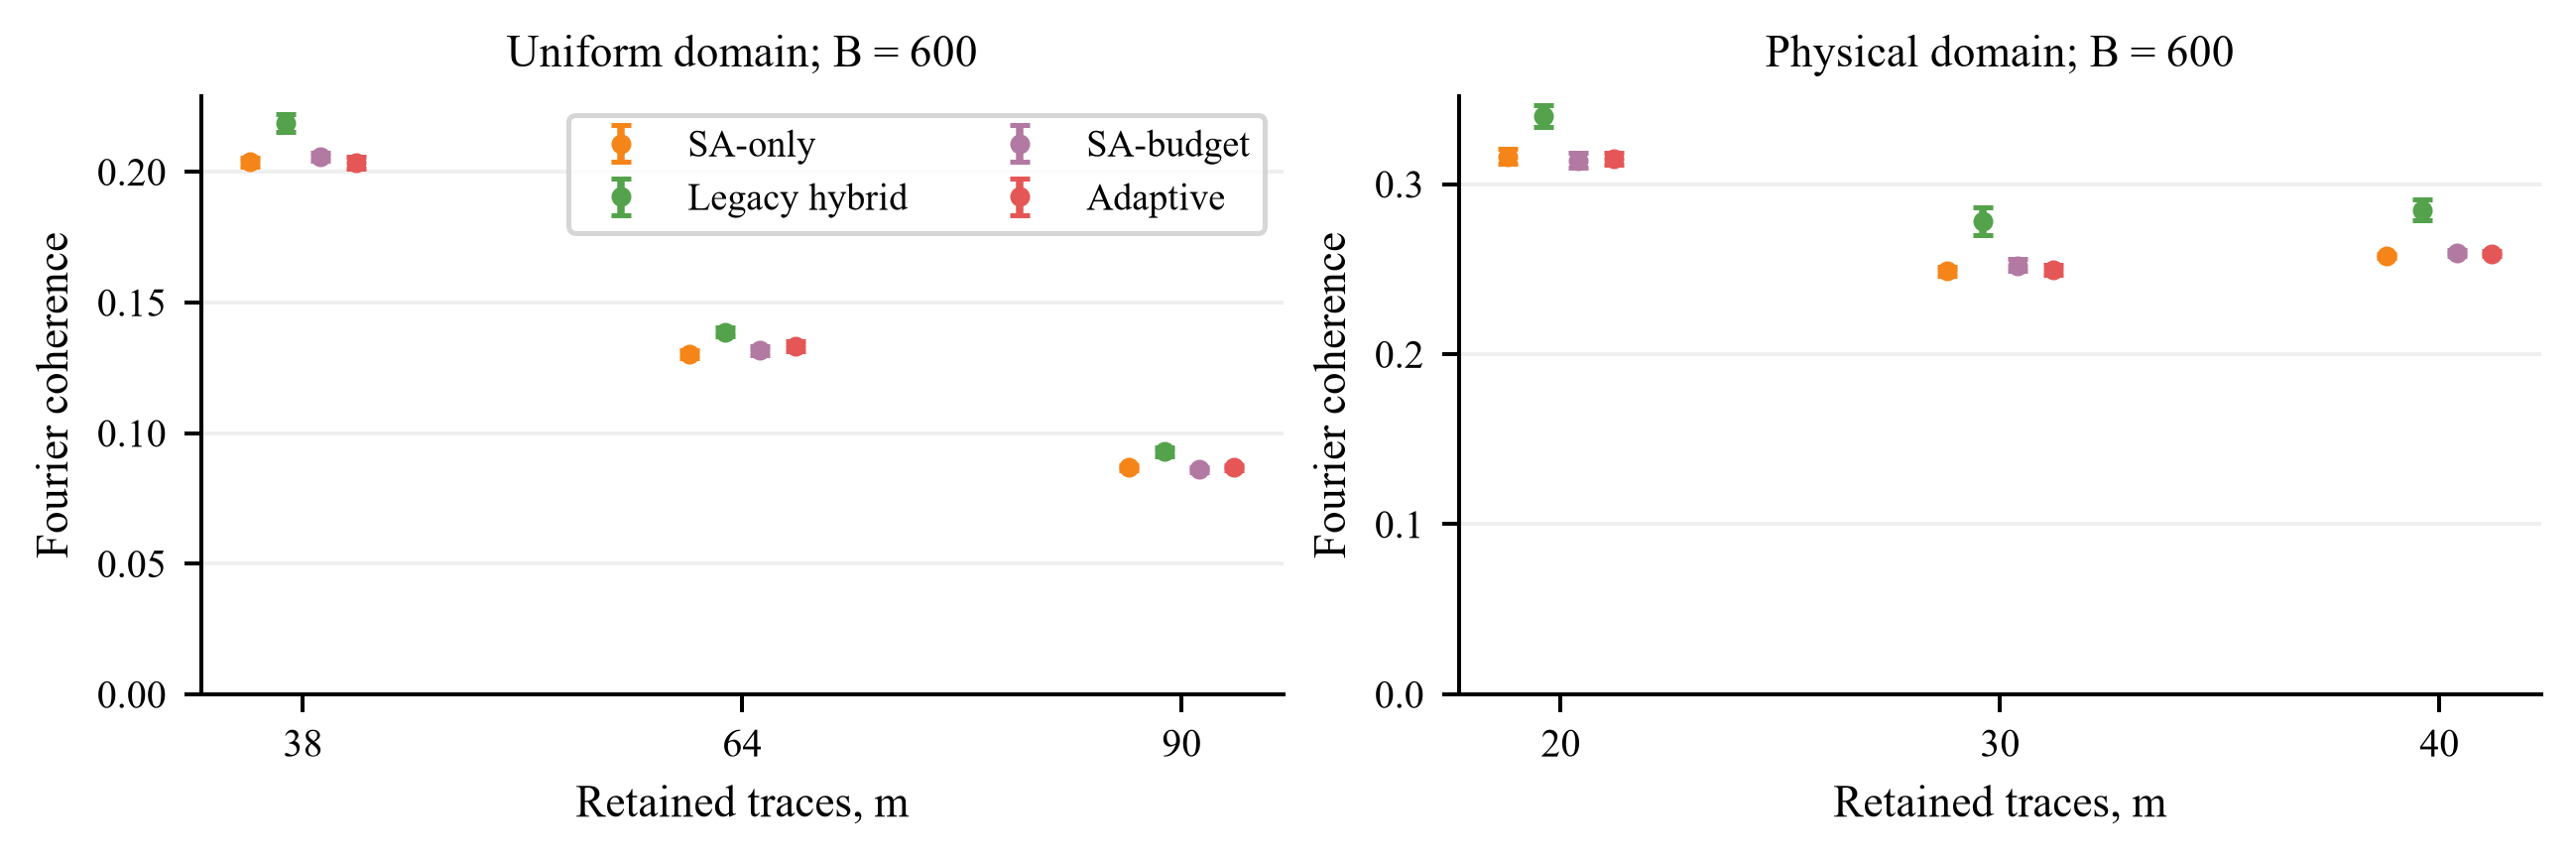
\includegraphics[width=\textwidth]{search.png}
\caption{Frozen v4 search at $B=600$: mean coherence and marginal 95\% bootstrap intervals across 20 seeds. Uniform counts are 38/64/90 of 128; physical counts are 20/30/40 of 59. All methods optimize the same unpenalized objective within a group. The physical interpretation remains conditional on header geometry.}
\label{fig:search}
\end{figure*}

For uniform $m=38$, $B=600$, the paired Adaptive-minus-hybrid difference is $-0.015055$, with 95\% bootstrap interval $[-0.019027,-0.011239]$, rank-biserial effect $-1$, and Holm-adjusted $p=0.0001373$ (Table~\ref{tab:search}). The corresponding Adaptive-minus-SA-only difference is $-0.000301$, with interval $[-0.003289,0.002413]$ and effect 0.0667. The sign convention is lower-is-better. A small favorable mean is not sufficient to claim a reliable algorithmic advantage.

\begin{table}[t]
\caption{V4 Uniform $m=38$, $B=600$: Adaptive Minus Reference}
\label{tab:search}
\centering\footnotesize\setlength{\tabcolsep}{3pt}
\begin{tabular}{lrrr}\toprule
Reference & Mean $\Delta\mu$ & Marginal 95\% CI & Holm $p$\\\midrule
\SearchContrastRows
\bottomrule\end{tabular}
\par\smallskip\parbox{\columnwidth}{Twenty paired seeds; 72-test correction family. Lower $\Delta\mu$ favors Adaptive. Rows are generated from the independent recomputation of the frozen result tables.}
\end{table}

\begin{figure*}[t]
\centering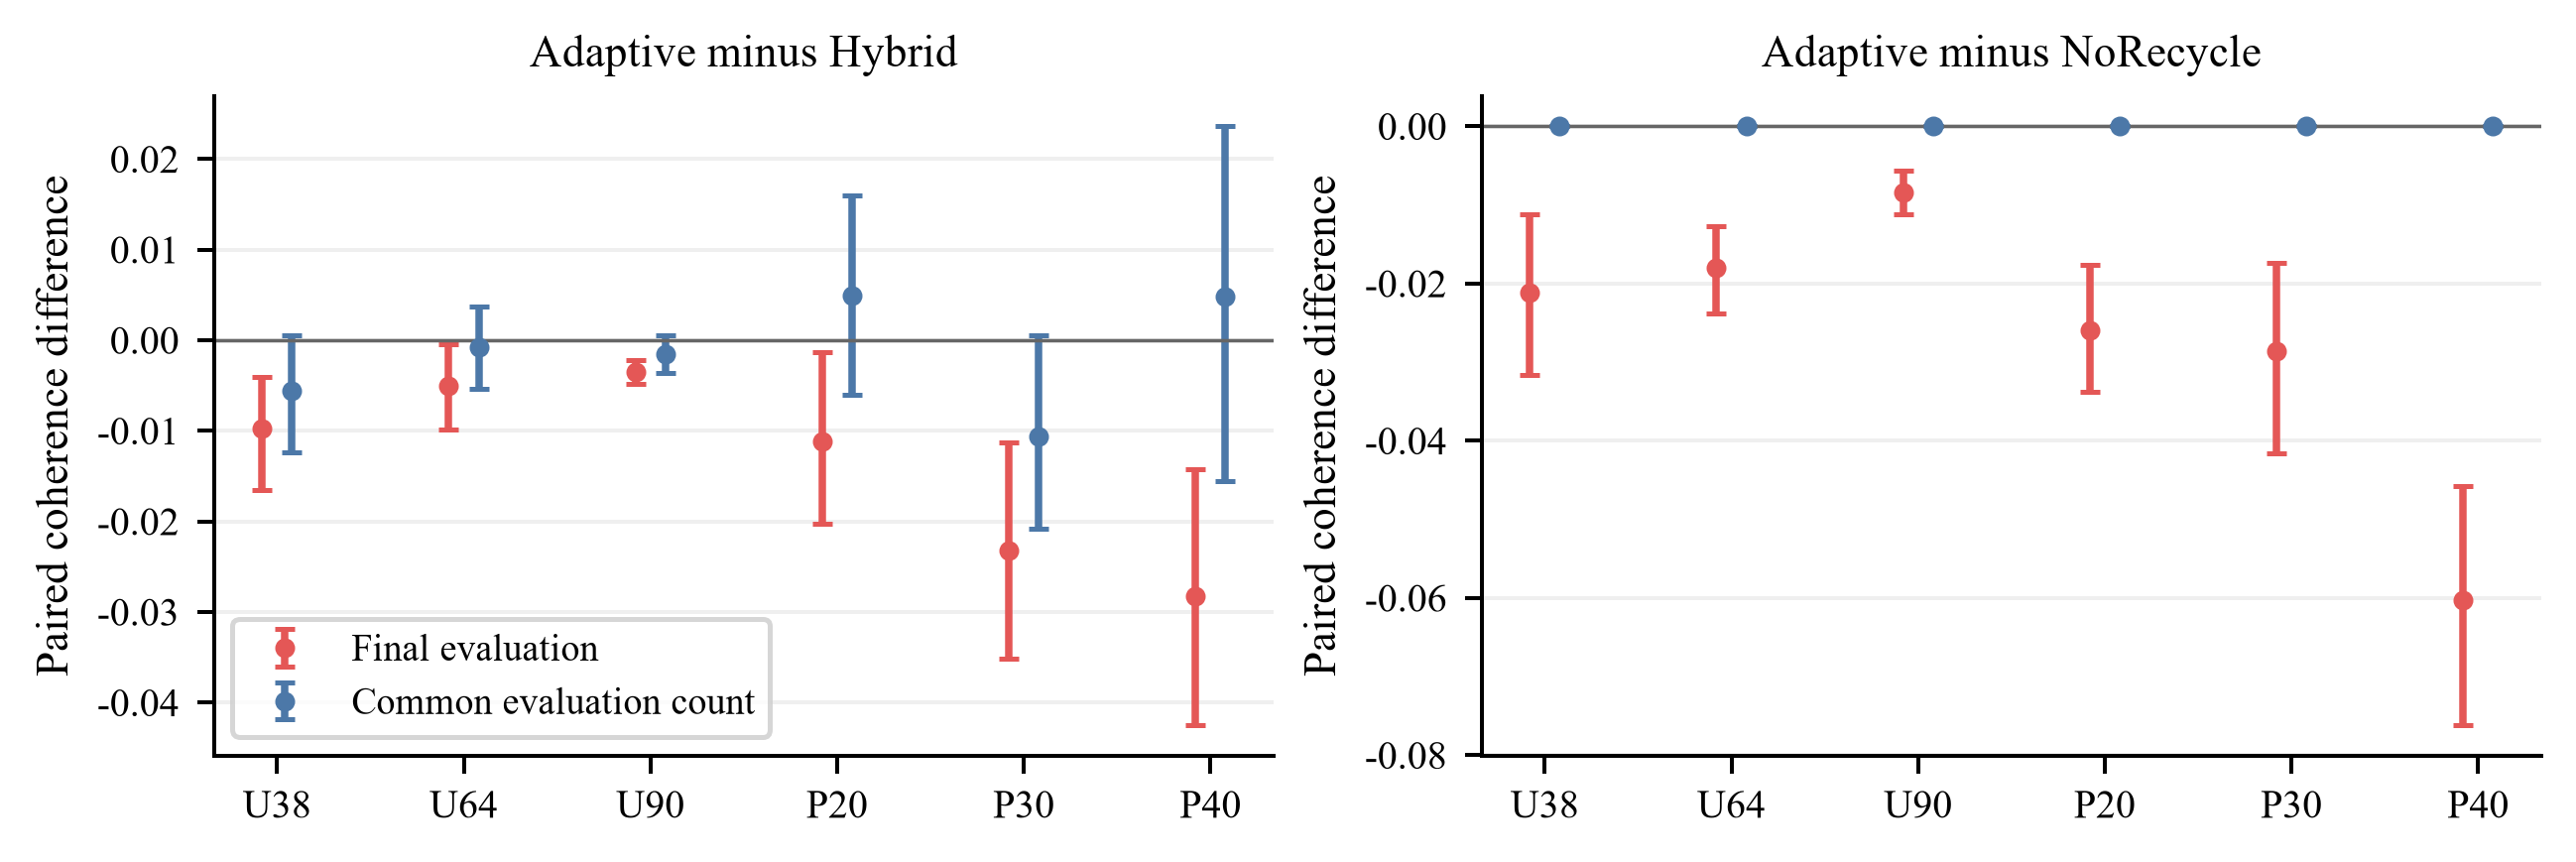
\includegraphics[width=\textwidth]{budget.png}
\caption{V5 paired coherence differences at $B=300$, ten seeds per group. U/P denote uniform/physical coordinates. Final-score differences and differences truncated to common actual evaluation counts are distinct. The Adaptive--NoRecycle common prefixes are exactly identical. Error bars are marginal bootstrap intervals; the 42-test Holm family has no significant contrasts.}
\label{fig:budget}
\end{figure*}

The v5 study produces no significant contrast in its 42-test family; the smallest adjusted $p$ is 0.08203125. With ten nonzero pairs, the smallest possible two-sided exact sign probability is $2/2^{10}$, and even multiplying this by 42 exceeds 0.05 for the first Holm rejection. The design therefore has insufficient resolution for that family, irrespective of an apparently large descriptive effect. It cannot establish the absence of useful switching or neighborhood effects.

The equal-count analysis is more directly diagnostic. Adaptive and NoRecycle are identical until the latter terminates; all six group mean differences over their common prefixes are exactly zero. Their final differences consequently include additional use of the remaining evaluations. Fig.~\ref{fig:budget} also shows that this attribution does not imply all other hybrids have identical prefixes. Independent universal benefits from switching, mixed neighborhoods, or extra perturbation remain unestablished. NoPerturb sometimes has a better descriptive mean and sometimes a worse one; it was not retrospectively promoted to the main method.

Under a 30-ms limit, mean measured search durations range from approximately 30.017 to 30.040 ms, with about 518--633 evaluations. Adaptive has favorable mean coherence in that setup. However, $B=100000$ remains the cooling reference, so none of these short runs completes its evaluation-based annealing schedule. Equal wall-clock limits do not imply matched cooling progress. These measurements are conditional timing diagnostics, not a universal speed claim. Shared-cache savings and search-policy effects must also be distinguished.

\subsection{Geometry and Missing-Trace Recovery}
Fig.~\ref{fig:recovery} separates fixed recovery from observed-only model selection on the common external set. For Adaptive, fixed-recovery mean SNRs are 10.3200, 12.5619, and 13.7482 dB for the three counts. Their six-template intervals are respectively [7.7316,12.4192], [11.0705,13.8434], and [12.1799,15.2168] dB. Selected-recovery means are 10.4690, 12.4396, and 13.7975 dB. Selection does not guarantee an external improvement: the middle-density Adaptive mean decreases after inner selection.

\begin{figure*}[t]
\centering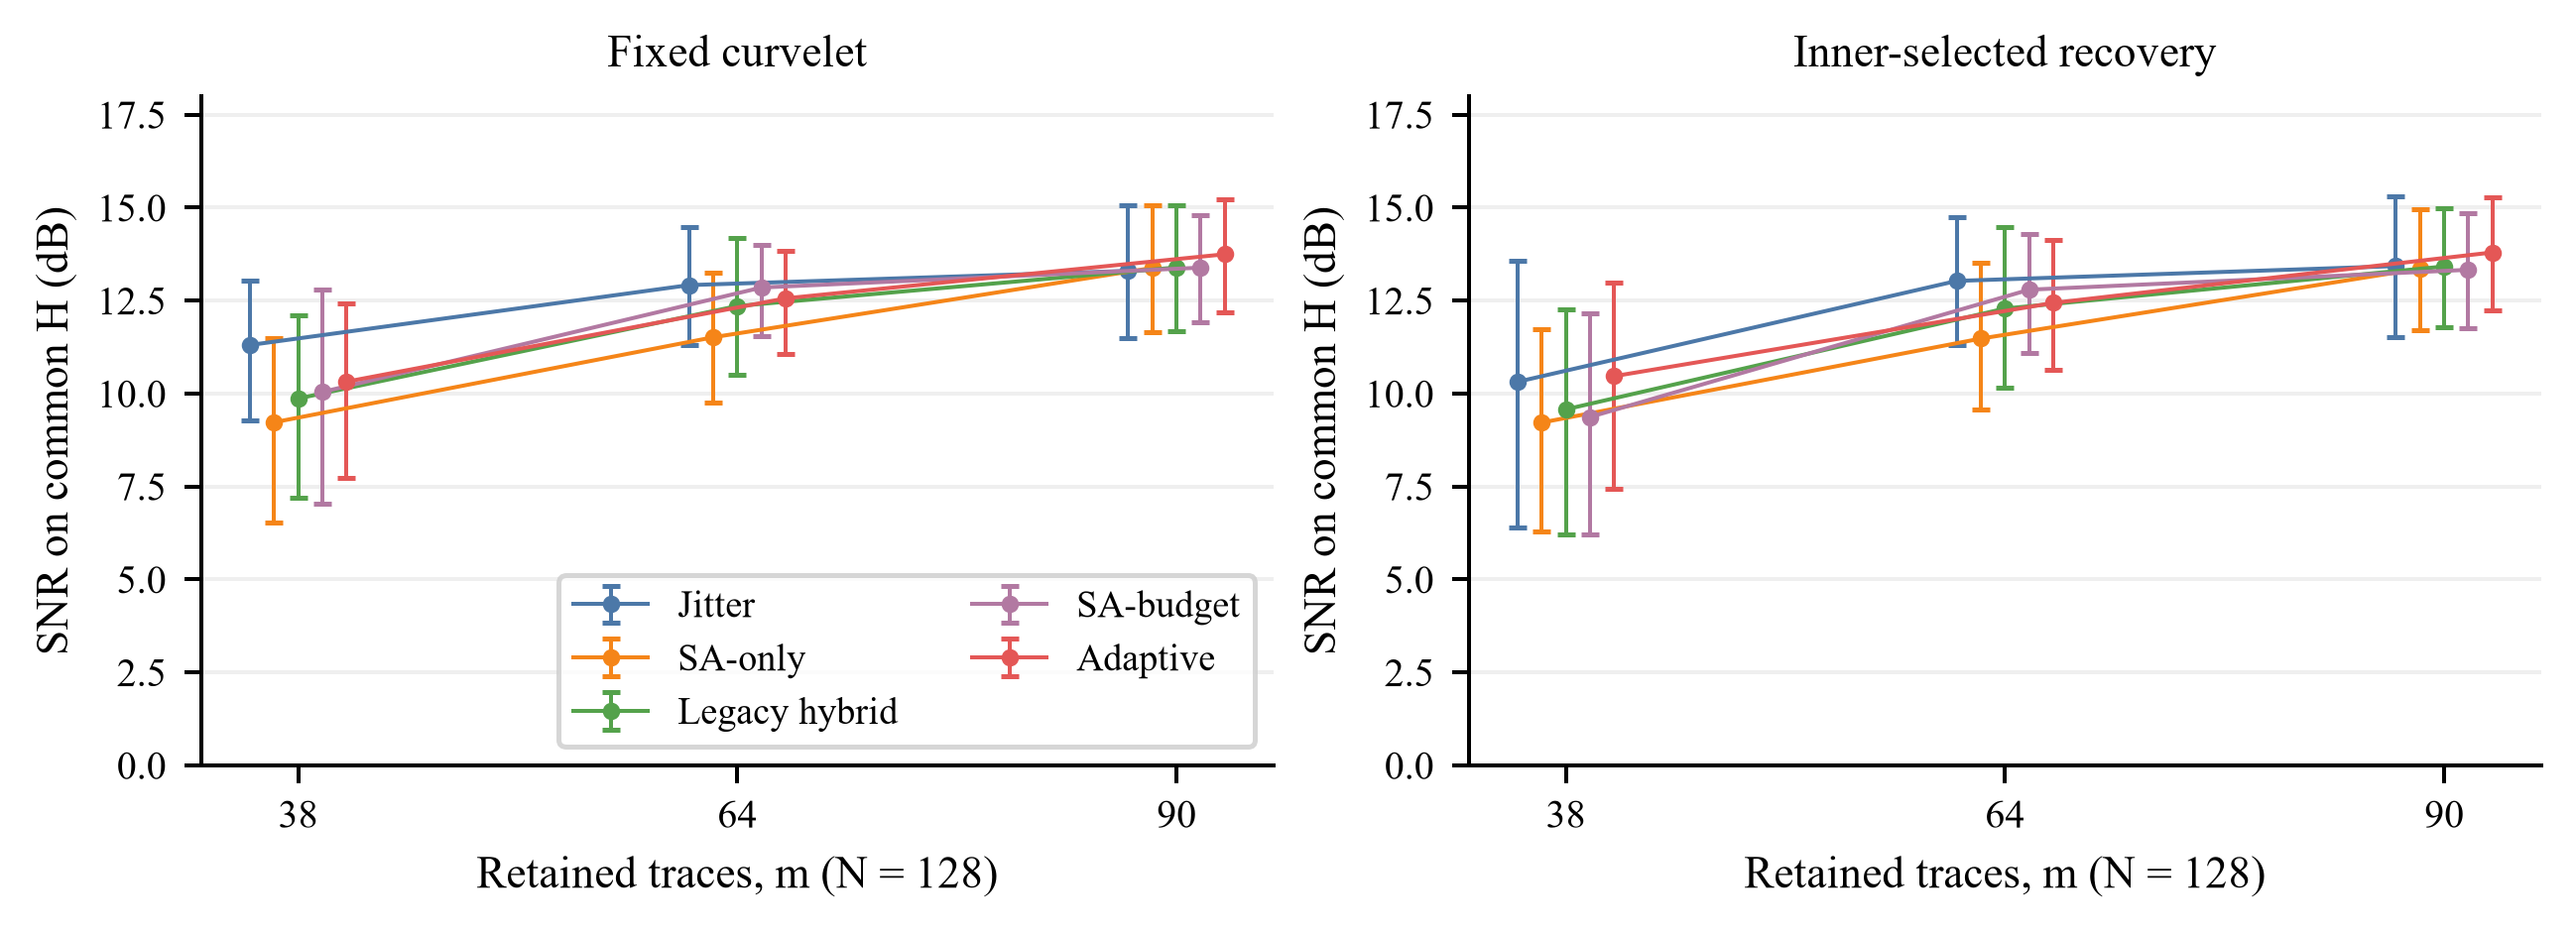
\includegraphics[width=\textwidth]{recovery.png}
\caption{Common-$H$ synthetic recovery. Means and marginal bootstrap intervals use six clean structural templates after averaging three mask seeds and two noise settings. The target includes the prescribed noise. Left: fixed curvelet recovery. Right: a frozen four-candidate recovery pool with observed-only validation and gain selection. No comparison survives the 24-test template-level Holm family.}
\label{fig:recovery}
\end{figure*}

At $m=38$, Adaptive minus Jitter under fixed recovery is $-0.9866$ dB, with marginal interval $[-1.9044,-0.2109]$, effect $-0.9048$, raw $p=0.0625$, and adjusted $p=1$. Adaptive minus SA-only is $+1.0924$ dB, with interval [0.5560,1.6493], effect 1, raw $p=0.03125$, and adjusted $p=0.75$. The 24-comparison family has no significant contrast: six nonzero pairs imply a first-step Holm resolution limit of $24(2/2^6)=0.75$. Nonzero marginal intervals and nonsignificant family-adjusted tests are compatible; they answer different uncertainty questions. These limited deterministic templates do not establish a population-wide ranking.

\begin{table}[t]
\caption{Common-$H$ Fixed Recovery: Adaptive Minus Reference}
\label{tab:recovery}
\centering\footnotesize\setlength{\tabcolsep}{3pt}
\begin{tabular}{rlrrr}\toprule
$m$ & Reference & $\Delta$ dB & Marginal 95\% CI & Holm $p$\\\midrule
\RecoveryContrastRows
\bottomrule\end{tabular}
\par\smallskip\parbox{\columnwidth}{Six clean structural templates; each first averages three masks and two noise levels. Higher differences favor Adaptive. Adjustment uses the full 24-test family, including selected recovery and other references.}
\end{table}

Table~\ref{tab:recovery} gives additional common-$H$ contrasts. The traditional complement evaluation yields a different task. At $m=38$, fixed-recovery means for Jitter, SA-only, legacy hybrid, SA-budget, and Adaptive are 11.1534, 8.1287, 7.8681, 7.8271, and 8.6472 dB, respectively. These values should not be subtracted from common-$H$ scores as a methodological gain because the targets differ. The common-$H$ experiment controls evaluation locations but constrains acquisition eligibility; neither design replaces the other.

Across unique masks within each structure/noise condition, coherence--SNR Spearman correlations change sign. In the common-$H$ design, ranges are $[-0.154,0.511]$, $[-0.448,0.576]$, and $[-0.897,0.509]$ across the three densities. Maximum gap and nearest-neighbor variation are also retained in the descriptive association analysis. This conditional heterogeneity supports proxy mismatch, not a causal explanation for every mask. Coverage weighting can improve some recoveries, as seen in the retained nine-weight v4 study, but its geometric Pareto tradeoff does not demonstrate universal recovery improvement or justify choosing weights using hidden SNR.

\subsection{Conditional Real-Data Results and Isolation}
Fig.~\ref{fig:real} retains all preset windows and both splits. Seventeen of 24 default recoveries have negative SNR, compared with one after inner selection; zero prediction is not selected in these 24 cases. For the full native record, fixed means at 20/30/40 retained traces are $-0.2745$, 0.2962, and 0.9441 dB, versus 0.3480, 0.6702, and 1.1809 dB after selection. These are modest prediction scores conditional on unconfirmed decoding, not evidence of calibrated high-fidelity wavefield recovery.

\begin{figure*}[t]
\centering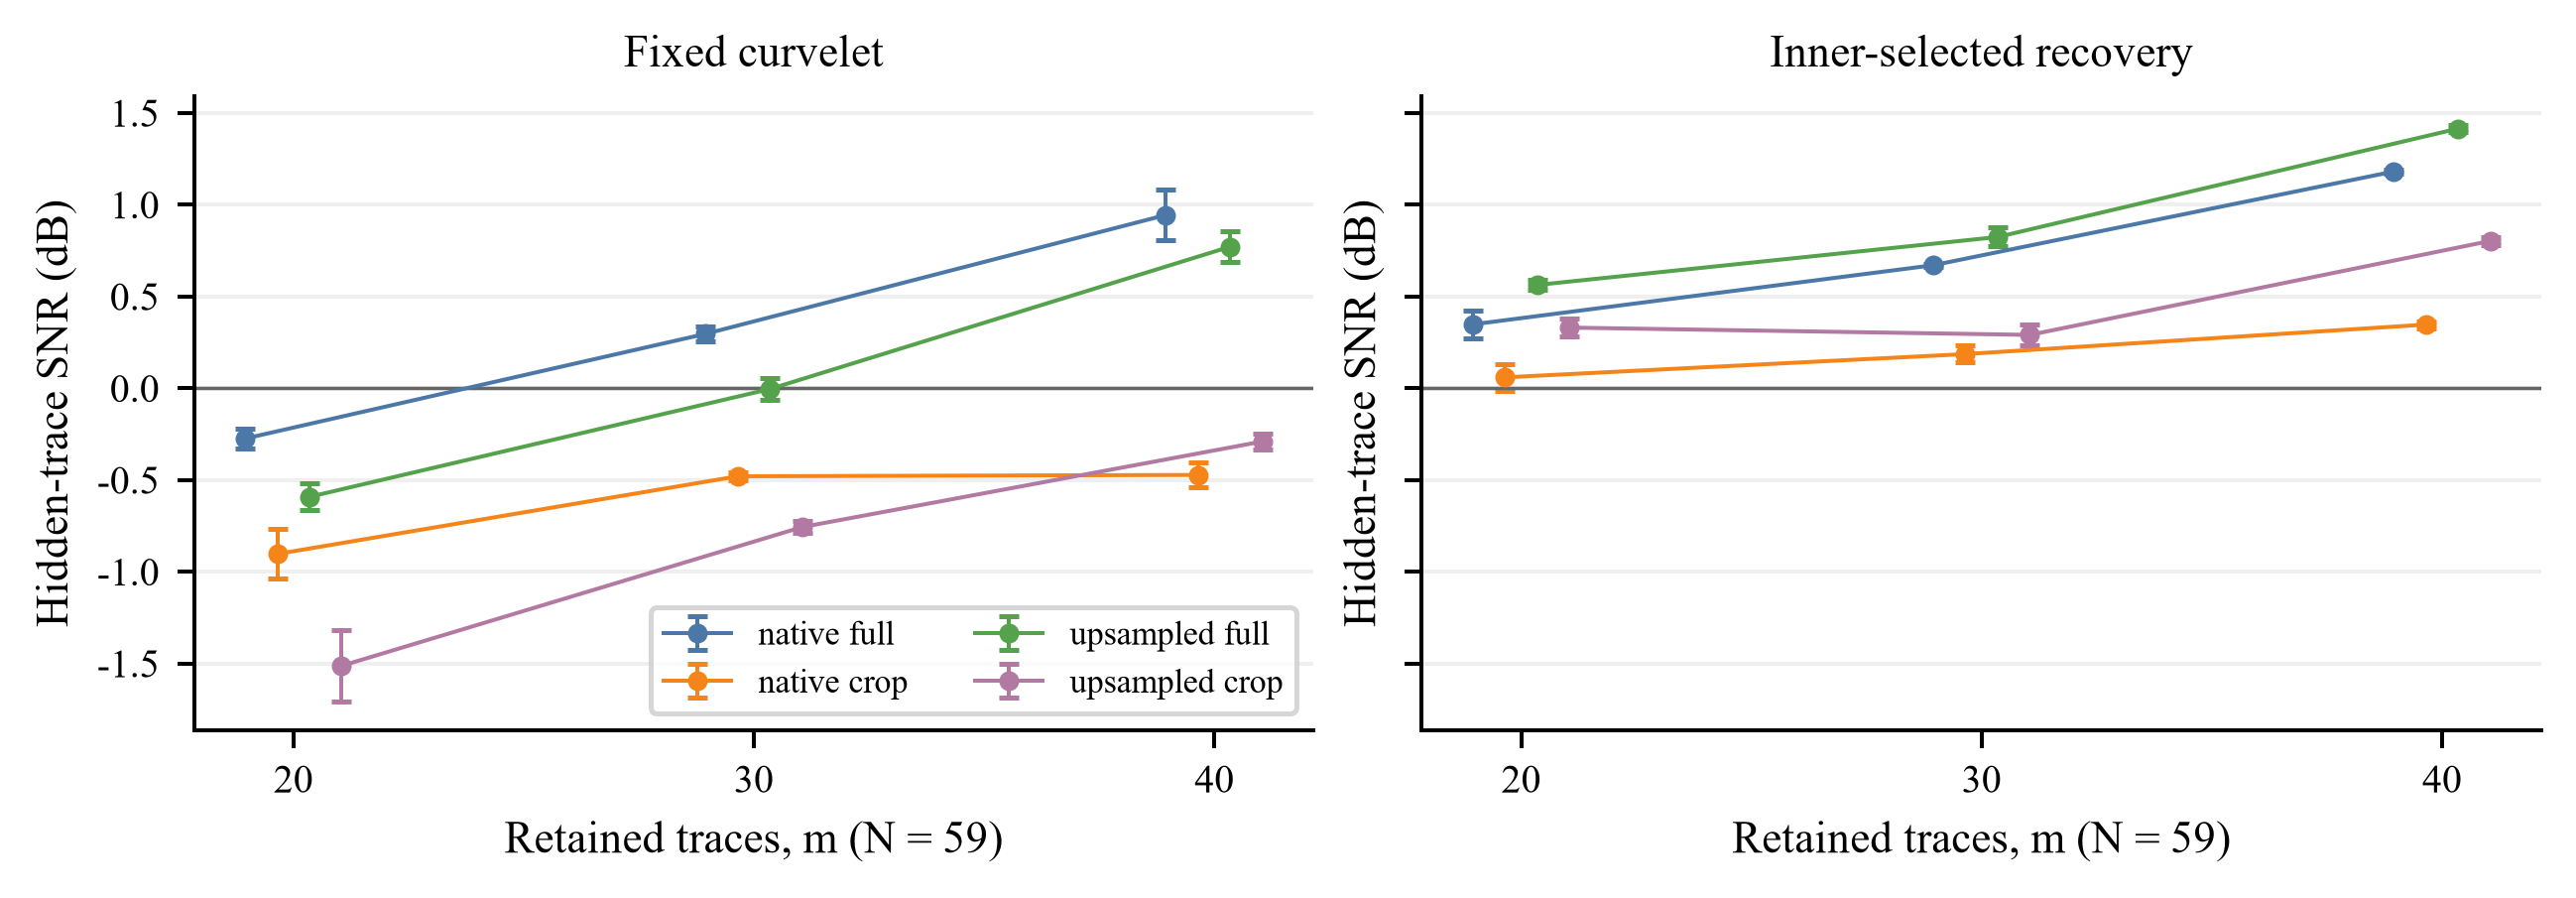
\includegraphics[width=\textwidth]{real_windows.png}
\caption{One real source under the unconfirmed IEEE-LE payload interpretation. Points average two common geometric splits; bars show their observed minimum--maximum range, not confidence intervals. Window and temporal-resampling sensitivities are all retained. The horizontal zero line is the zero-prediction SNR. Different windows have different targets and cannot be ranked as same-task gains.}
\label{fig:real}
\end{figure*}

The prediction-error identity offers a useful diagnostic. For hidden truth $y$ and prediction $p$,
\begin{equation}
\frac{\|p-y\|^2}{\|y\|^2}
=1+\frac{\|p\|^2}{\|y\|^2}-2\frac{\langle p,y\rangle}{\|y\|^2}.
\end{equation}
High prediction energy with a small cross term can produce a negative SNR even when observations are fitted accurately. Inner gain shrinkage can reduce this error without preserving event amplitudes. Weak training-trace continuity, array-scale mismatch, mixed CDPs, extrapolation, and nonlinear iteration are plausible contributors, but this identity does not identify a unique cause. Encoding and acquisition-history uncertainty prevent assigning the failure to a single processing bug or adopting unverified normal-moveout correction.

An end-to-end hidden-amplitude intervention replaces withheld values by $13y+7$. In the v5 raw-amplitude chain, the selected model is unchanged and the maximum prediction difference is exactly zero in the archived check. A historical globally normalized chain is not strictly isolated: after CSV rounding, the corresponding original-unit prediction difference is about 0.007482, or $1.046\times10^{-6}$ of the original numerical peak 7155. An earlier text incorrectly described that relative factor as the peak itself; this audit corrects the description. Small dependence is not zero dependence. The new chain removes the global pre-holdout normalization rather than explaining it away by idealized scale cancellation.

\section{Reproducibility, Limitations, and Implications}
Independent checks distinguish implementation fidelity from scientific suitability. Explicit NumPy dictionaries and small-mask enumeration verify coherence, coverage, and hard feasibility in 588 cases. Dense coordinate-projection references verify two native cases. Twenty FDCT parameter/size combinations in each of Release and Debug have maximum relative inverse-transform error below $2.30\times10^{-15}$. These results establish numerical agreement over tested cases; they do not guarantee missing-trace accuracy. A scale-aware observation-consistency check repairs an input-unit failure without changing the archived search/recovery conclusions.

The current-code validation checks both native builds, complete regressions, Python tests, historical archives, and replay of 930 searches and six preset recovery predictions. Replay equality excludes nondeterministic timing fields. Commands, configurations, seeds, executable/source/input/output hashes, and original outputs are preserved. Native GUI screenshots test startup and selected dialogs but do not replace a complete manual interaction audit. Results from v2, v3, v4, and v5 remain separate, and generated paper figures use archived numerical tables rather than manually entered favorable values.

Several limitations govern interpretation. First, the real source's header structure is supported, but the sample encoding, physical units, grouping, and coordinate scaling remain unresolved. Source-matched export metadata and known numerical samples from the provider are needed. Second, six prescribed analytic templates and one conditional real source do not establish cross-survey generalization. Additional masks or noise settings cannot substitute for independent geology. Third, the studies compare a constrained set of search and recovery baselines; modern signal-adaptive or learned methods are not benchmarked. No state-of-the-art performance claim follows.

Fourth, exact small-sample testing is coarse. The 42-test ten-seed search family and the 24-test six-template recovery family cannot support broad confirmatory conclusions. Dependence was corrected transparently after initial analysis, not concealed. Fifth, the current time-limit test confounds incomplete cooling with phase behavior, and the implementation has only been fully checked in its recorded Windows/VS2008/Qt4 environment. Sixth, the recovery objective is pointwise error on hidden noisy traces. Phase, amplitude, moveout, and downstream imaging fidelity require separate measures and independently justified data.

The practical implication is to retain the simplest supported mechanisms. Budget recycling prevents a documented form of premature termination; the evidence does not require presenting every switch or perturbation as independently beneficial. Fourier coherence remains a useful reproducible geometric descriptor, but coverage, signal structure, solver configuration, and acquisition semantics must accompany it. A future signal-dependent objective should be defined from permitted training information or a prespecified physical model, followed by a new frozen validation protocol. Increasing seeds until significance appears or choosing a preprocessing window from external SNR would not resolve the present limitations.

\balance
\section{Conclusion}
A fixed-cardinality, budget-aware hybrid trace selector was implemented and evaluated with physical Fourier coherence and explicit spatial coverage. It improves the legacy hybrid's final mean geometric objective in the frozen comparisons, while stable superiority over SA-only remains unsupported. Identical Adaptive--NoRecycle prefixes show that continued use of the allowed evaluations is the clearest mechanism-level explanation. Common external holdouts and observed-only recovery selection reveal that geometric improvement and reconstruction improvement are separate claims. The six-template joint study and conditional real-data diagnostics do not establish universal recovery gains or high-fidelity real-data reconstruction. The resulting contribution is a reproducible, budget-accounted selection and validation workflow with explicit negative evidence and clearly delimited data assumptions.

\section*{Data and Code Availability}
The accompanying project contains versioned native/Python sources, original result tables, commands, masks, predictions, provenance manifests, independent statistical recomputation, and a reproducible manuscript build. The source baseline is Git \texttt{8b9ffef}; modifications for this manuscript are additionally identified by file hashes. The real file is identified by SHA-256 \texttt{ddcb311b2406af17}\allowbreak\texttt{cf375b570b3eb8ea}\allowbreak\texttt{7ca2d81cdeb002f97}\allowbreak\texttt{2e6d668cd7b2bc2}. A public repository URL and redistribution authorization are not supplied; external reproducibility and data access must be resolved before submission. No data license is inferred from local possession.

\section*{Acknowledgment}
OpenAI Codex assisted in drafting the abstract and Sections I--VII and in preparing verification, plotting, and manuscript-build scripts. Figures 1--4 are deterministic plots of archived numerical data. Responsibility for final scientific verification and submission remains with the author.

\begin{thebibliography}{10}
\bibitem{donoho} D. L. Donoho, ``Compressed sensing,'' \emph{IEEE Trans. Inf. Theory}, vol. 52, no. 4, pp. 1289--1306, 2006, doi: 10.1109/TIT.2006.871582.
\bibitem{candes} E. J. Cand\`es, J. K. Romberg, and T. Tao, ``Stable signal recovery from incomplete and inaccurate measurements,'' \emph{Commun. Pure Appl. Math.}, vol. 59, no. 8, pp. 1207--1223, 2006, doi: 10.1002/cpa.20124.
\bibitem{jitter} G. Hennenfent and F. J. Herrmann, ``Simply denoise: Wavefield reconstruction via jittered undersampling,'' \emph{Geophysics}, vol. 73, no. 3, pp. V19--V28, 2008, doi: 10.1190/1.2841038.
\bibitem{crsi} F. J. Herrmann and G. Hennenfent, ``Non-parametric seismic data recovery with curvelet frames,'' \emph{Geophys. J. Int.}, vol. 173, no. 1, pp. 233--248, 2008, doi: 10.1111/j.1365-246X.2007.03698.x.
\bibitem{fdct} E. Cand\`es, L. Demanet, D. Donoho, and L. Ying, ``Fast discrete curvelet transforms,'' \emph{Multiscale Model. Simul.}, vol. 5, no. 3, pp. 861--899, 2006, doi: 10.1137/05064182X.
\bibitem{sa} S. Kirkpatrick, C. D. Gelatt, Jr., and M. P. Vecchi, ``Optimization by simulated annealing,'' \emph{Science}, vol. 220, no. 4598, pp. 671--680, 1983, doi: 10.1126/science.220.4598.671.
\bibitem{ils} H. R. Louren\c{c}o, O. C. Martin, and T. St\"utzle, ``Iterated local search,'' 2001, arXiv:math/0102188. [Online]. Available: \url{https://arxiv.org/abs/math/0102188}
\bibitem{holm} S. Holm, ``A simple sequentially rejective multiple test procedure,'' \emph{Scand. J. Statist.}, vol. 6, no. 2, pp. 65--70, 1979.
\bibitem{segy} SEG Technical Standards Committee, \emph{SEG-Y Revision 2.0 Data Exchange Format}, Jan. 2017, rev. Mar. 2017. [Online]. Available: \url{https://seg.org/wp-content/uploads/2025/11/seg_y_rev2_0_mar2017.pdf}
\end{thebibliography}
\end{document}
